\documentclass[crop,tikz]{standalone}
\usepackage{amsmath}
\usetikzlibrary{arrows}
\usetikzlibrary{positioning}
\usetikzlibrary{shapes}
\usetikzlibrary{hobby}
\usepackage[draft]{tikzpeople}

\newcommand\irregularcircle[2]{% radius, irregularity
  +(0:{(#1)+rand*(#2)})
  \foreach \a in {10,20,...,350}{
    -- +(\a:{(#1)+rand*(#2)})
  } -- cycle
}

\begin{document}
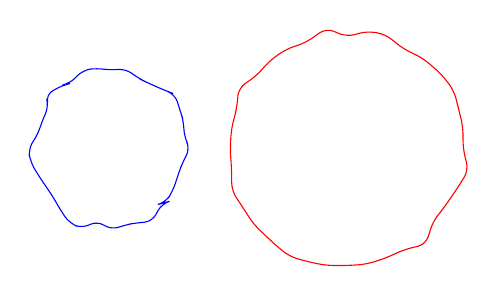
\begin{tikzpicture}
  \tikzset{line/.style={draw, <->, >=latex'}}
  \tikzset{line2/.style={draw, ->, >=latex'}}
  \tikzset{line3/.style={draw, <->, >=latex', dashed}}

  \coordinate (c) at (0,0);
  \coordinate (d) at (3,0);
  \draw[blue,rounded corners=1mm] (c) \irregularcircle{1cm}{1mm};
  \draw[red,rounded corners=1mm] (d) \irregularcircle{1.5cm}{1mm};

  % \node at (3,1.5) {Server state};
  % \node at (0,1.5) {Abstract machine};

\end{tikzpicture}
\end{document}